\lecture{2}{19.04.2017}{Dr. Raphael Kruse}{Frank Rehfeld}
\textbf{Wiederholung}\\
\begin{enumerate}
\item	
	$\begin{cases}
			u\colon\W=\left(a,b\right)\to\R\\
			\int_{\W}u^{\prime}\left(x\right)v^{\prime}\left(x\right)\,\mathrm{d}x = \int_{\W}f\left(x\right)v\left(x\right)\,\mathrm{d}x\\
			u\left(a\right)=u\left(b\right)
		\end{cases}$
\item{}
	Eigenschaften $\L^{p}$:\\
	\begin{itemize}
		\item $1\leq p <\infty \implies \L^{p}\text{ separabel}$
		\item $\L^{\infty}$ nicht separabel
		\item $1 < p <\infty, \frac{1}{p}+\frac{1}{q}=1 \implies \left(\L^{p}\right)^{\prime} \equiv \L^{q}$\\
			  $T\colon \L^{q}\to\left(\L^{p}\right)^{\prime}, \left(Tg\right)f = \int_{\W}f\left(x\right)g\left(x\right)\,\mathrm{d}x$
		\item $\left(\L^{1}\right)^{\prime}\equiv\L^{\infty}, \L^{1}\subsetneq\left(\L^{\infty}\right)^{\prime}$\\
				$\implies \L^{1}, \L^{\infty}$ sind nicht reflexiv
	\end{itemize}
\end{enumerate}

\begin{definition}
	$\L^{1}_{\text{loc}}\left(\W\right) := \left\{u\colon\W\to\R\colon u|_{K}\in\L^{1}\left(K\right)\forall K\subset\W \text{ kompakt}\right\}$\\
	\underline{Raum der lokal integrierbaren Abbildungen}
\end{definition}

\begin{definition}
	$\C^{\infty}_{\text{c}}\left(\W\right) := \left\{f\colon\W\to\R\colon f\in\C^{\infty},\operatorname{supp}\left(f\right)\subset\W\text{ kompakt}\right\}$\\
	\underline{Raum der unendlich oft differenzierbaren Funktionen mit kompakten Träger}\\
	$\operatorname{supp}\left(f\right):=\left\{x\in\W\colon f\left(x\right)\neq 0\right\}$\\
	\boldmath$C^{\infty}_{\text{c}}\neq \C^{\infty}_{0}$
\end{definition}

\begin{expl}
	$\W=\R^{d},d\in\mathbb{N}$\\
	Glättungskern $J\left(x\right)=\begin{cases}
		\operatorname{exp}\left(-\frac{1}{1-|x|^{2}}\right) &, |x| < 1\\
		0 &, |x| \geq 1
	\end{cases}$
\end{expl}

\begin{definition}
	$u,v\in\L^{1}_{\text{loc}}$. Es gelte
	\begin{equation*}
		\int_{\W}u\left(x\right)\phi\left(x\right)\,\mathrm{d}x = -\int_{\W}v\left(x\right)\phi^{\prime}\left(x\right)\,\mathrm{d}x \forall\phi\in\C^{\infty}_{\text{c}}
	\end{equation*}
	$u$ heißt \underline{schwache Ableitung} von $v$, $v$ heißt \underline{schwach differenzierbar}
\end{definition}

\begin{expl}
	\begin{enumerate}
		\item{}
			$u\left(x\right) = |x|$ schwach differenzierbar auf $\left(-1,1\right)$\\
			$u^{\prime}\left(x\right) = \begin{cases}
				-1 &, x<0\\
				1 &, x>0
			\end{cases}$
		\item Heaviside-Funktion auf $\W = \left(-1,1\right)$\\
			$H\colon\W\to\R, x\mapsto\begin{cases}
				1 &, x>0\\
				0 &, x\leq 0
			\end{cases}$ ist nicht schwach differenzierbar
	\end{enumerate}
\end{expl}

\textbf{Eigenschaften}:
\begin{itemize}
	\item klassisch differenzierbar $\implies$ schwach differenzierbar
	\item schwache Ableitung ist eindeutig im $\L^{1}$-Sinne
	\item übliche Eigenschaften (Linearitär,...) bleiben erhalten
\end{itemize}

\begin{lemma}[Fundamentallemma der Variationsrechnung]
	Sei $u\in\L^{1}_{\text{loc}}$ und
	\begin{equation*}
		\int_{\W}u\left(x\right)\phi\left(x\right)\,\mathrm{d}x = 0 \forall\phi\in\C^{\infty}_{\text{c}}
	\end{equation*}
	so folgt $u=0\in\L^{1}_{\text{loc}}$.
\end{lemma}

\begin{multicols}{2}
\begin{definition}
	$J_{\e}\colon\R\to\R, J_{\e}\left(x\right)=\begin{cases}
		c_{\e}\operatorname{exp}\left(-\frac{\e^{2}}{\e^{2}-x^{2}}\right) &, x\in\left(-\e,\e\right)\\
		0 &, \text{ sonst}
	\end{cases}$\\
	$c_{\e}:=\left(\int_{\e}^{\e}\operatorname{exp}\left(-\frac{\e^{2}}{\e^{2}-x^{2}}\right)\,\mathrm{d}x\right)^{-1}$
	$J_{\e}$ ist der \underline{Standard-Glättungskern} mit Träger $\left[-\e,\e\right]${}
	\begin{itemize}
		\item $J_{\e}\in\C^{\infty}_{c}\left(\W\right)$
		\item $\int_{\R}J_{\e}\left(x\right)\,\mathrm{d}x = 1$
		\item $J_{\e}\left(x\right)\geq 0 \forall x\in\R$		
	\end{itemize}
	$\implies J_{\e}$ ist Wahrscheinlichkeits-Dichte
\end{definition}
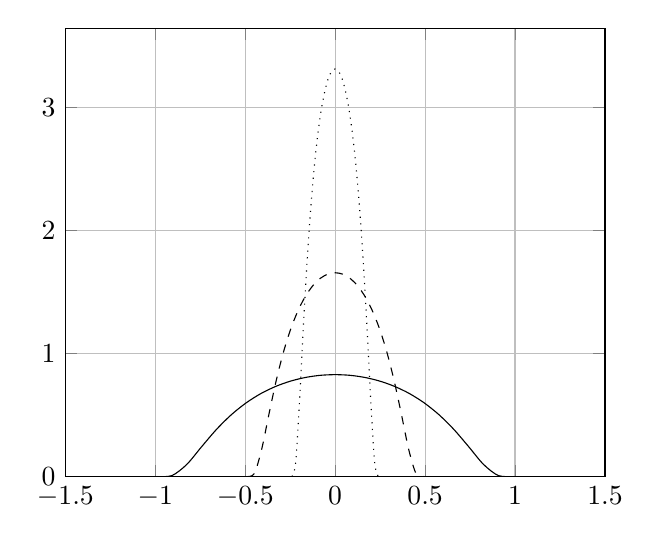
\begin{tikzpicture}
	\begin{axis}[scaled ticks=true,xmin=-1.5,xmax=1.5,ymin=0,grid=both]
		\addplot[domain=-0.99:0.99, smooth] {e^(-1/(1-x^2))/0.444};
		\addplot[domain=-0.49:0.49, style=dashed, smooth] {e^(-(1/4)/((1/4)-x^2))/0.222};
		\addplot[domain=-0.24:0.24, style=dotted, smooth] {e^(-(1/16)/((1/16)-x^2))/0.111};
	\end{axis}
\end{tikzpicture}
\end{multicols}
